\section{Detailed Architecture}
\label{DetailedArchitecture}
In this Section we introduce the tool we use to realize the chosen methodological approach. In addition, we describe the constraints under which we carry out the transformation, such as the use of a BPEL subset and the specification of a workflow pattern.
Later in this Section, we introduce the design ideas of our transformation and the general architecture we adopted.\\

FIXME: TO REMOVE LATER
\begin{itemize}
 \item *The M2T tool we use (Acceleo)
 %\item The additional components (A WebService)
\end{itemize}

The main points and some more decision we have to take over:
\begin{itemize}
  \item * We identify the subset of BPEL instructions suitable for a proof of concept of the transformation. 
  \subitem * Select a BPEL meta-model that covers the chosen subset of instructions.
  \subitem * Individuate a BPEL workflow pattern to work on 
 
 \item Provide a transformation strategy from the BPEL constructs to Java concepts
 \item Design the structure of the output application.
 \item Define the essential skeleton of Java classes necessary to create a runnable BPEL process
 \item the usage of the wsdl-to-java routine to create the tree of messages types
 \item In the templates, describe how to use and where the dynamic information taken from the BPEL input model has to be placed.
 \item Plan where and how, in the architecture, the developer intervention has to take place.
 \item \textbf{Issues encountered and proposed solutions  ?}
\end{itemize} 
 
 To mention later: \\
 StubPartnerLinks, code to be input by the user, static code, the problem with the WSDL file

\begin{itemize}
 \item Metamodel 
 \item Skeleton 
 \item Generator 
\end{itemize}

%//////////////////////////////////////////////////////////
\subsection{The M2T Generator}
To implement our model-to-text methodology we make use of the Acceleo generator. As described in Section \ref{acceleo}, Acceleo takes as input a model in any kind of modeling language followed by its meta-model descriptor, and a series of templates defining the structure of the output text to create.
With a well defined Acceleo transformations, we can obtain runnable 
Acceleo provides us the opportunity to both navigate the parameterized input model and to plan the design of the Java templates in order not to have redundant code.
%//////////////////////////////////////////////////////////
\subsection{The BPEL subset of instructions}
\label{Sec:BPELsubset}
The BPEL standard (see Section \ref{BPEL} for more details) has a wide variety of elements and instructions aimed at managing the possible workflow patterns obtainable during a services orchestration. Moreover, BPEL does not restrict the number of services that can participate to the orchestration neither the type and the quantity of interactions among them.
For these reason, we focus our attention on a subset of the whole BPEL language, both to restrain the complexity and to fit the time frame of the project.
\subsubsection{The activities subset}
We decided to restrict the BPEL activities to a subset containing the following constructs divided in four groups:
\begin{center}
\begin{supertabular}{p{0.4\textwidth}p{0.4\textwidth}}

1. Basic activities: 			& 2. Structured activities:		\\
\begin{itemize}
	\item \verb|<invoke>|
	\item \verb|<receive>|
	\item \verb|<reply>|
	\item \verb|<assign>|
	\end{itemize} 			&

					    \begin{itemize}
					      \item \verb|<sequence>|
					     \end{itemize}			\\
					     
3. Elementary operations: 		& 4. Static descriptive elements:	\\					
\begin{itemize}
	\item \verb|<copy>|
	\item \verb|<from>|
	\item \verb|<to>|
  \end{itemize} &

					    \begin{itemize}
					      \item \verb|<process>|
					      \item \verb|<partnerLink>|
					      \item \verb|<variable>|
					      \item \verb|<expression>|
					    \end{itemize}\\
\end{supertabular}
\end{center}

The Basic and Structured activities define the BPEL process logic (see Section \ref{BPELActivities}). The elementary operations are present inside the activities, while the static descriptive elements are meant to statically describe some of the parameters needed by BPEL process.
These elements allow the creation of simple BPEL processes, where the activities such as: invoking a service or waiting for a reply, happen as a sequence, one after the other. Although this limits the expressive potentiality of BPEL, it fits our need of focusing on proving the feasibility of an automated transformation from BPEL to Java without having to deal with the complexity of the whole language.
In Figure \ref{fig:SubSetBPEL} the BPEL subset of elements used for this project is depicted.

\begin{figure}
  \begin{center}
    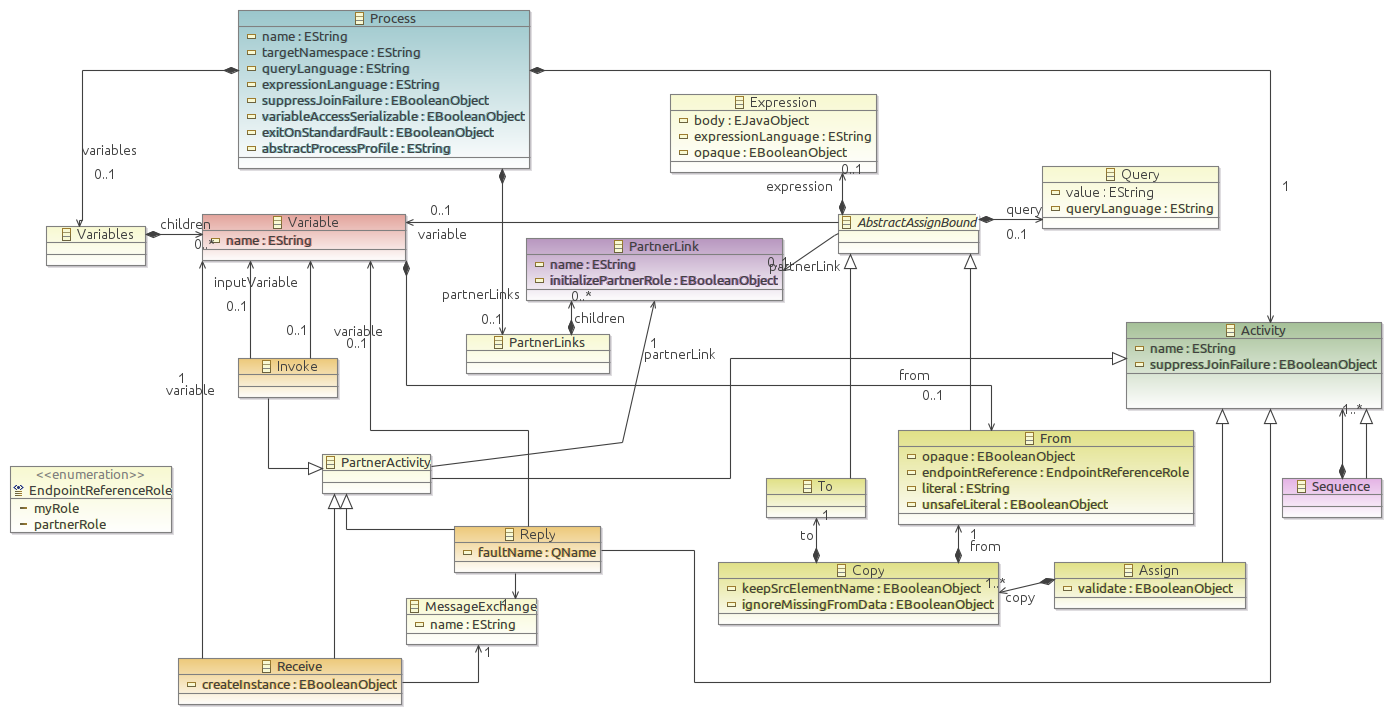
\includegraphics[scale=0.67,angle=90]{pictures/SubSetBpel2.png}
    \caption{The BPEL subset in its ecore model representation}
    \label{fig:SubSetBPEL}
  \end{center}
\end{figure} 

\subsubsection{The meta-model for the BPEL subset}
\label{Sec:DesignBpelSubset}
To permit the parameterization of the BPEL process input model, we need a meta-model describing our subset. The Eclipse Modeling Framework (see Section \ref{EMF}) provides a meta-model written in ecore for the whole BPEL language; we use only the subset elements of this ecore meta-model.
\subsubsection{The BPEL workflow pattern to focus on}
\label{sec:DesignBPELPattern}
The BPEL language with its wide range of activities and operation, gives the possibility to orchestrate many kind of workflow patterns among the participant services. We concentrate our attention on a process having the following participants:
\begin{itemize}
 \item one partner link representing a client
 \item one partner link describing a web-service
\end{itemize}
and on a simple workflow pattern that concerns the activities shown in Figure: \ref{fig:BPELWorkflowPattern}\footnote{This Figure has been realized using the BPEL designer facilities of Eclipse. Yet not a standard, as the Oasis consortium has not released a graphical standard, many vendors provide very similar graphical notations}. The pattern shown in the Figure includes the following steps:
\begin{enumerate}
 \item the process waits for a client to connect and provide an input
\item reception of the input and its assignation to a variable to forward to the web-service.
\item web-service invocation
\item reception of the web-service's reply and assignation to a variable to be forwarded back to the client
\item final response sent back to the client
\end{enumerate}


\begin{figure}
  \begin{center}
    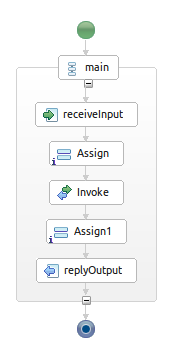
\includegraphics[scale=0.8]{pictures/BPELSimpleProcess.png}
    \caption{The BPEL workflow pattern we focus on}
    \label{fig:BPELWorkflowPattern}
  \end{center}
\end{figure} 

%///////////////////////////////////////////////////////////////
\subsection{Transformation Strategy}
\label{sec:TransformationStrategy}
As a direct transformation from BPEL constructs in Java concepts is neither feasible nor advisable, we have to provide a general strategy tackling single or groups of BPEL activities and creating Java counterparts. The following sections describe the single components of this strategy.

\subsubsection{The input files we work on}
\label{sec:inputFiles}
In a simple BPEL process there are two kind of files containing data valuable for our transformation: the BPEL process description files and the WSDL files to describe the services the process is orchestrating.
The BPEL process files contain: 
\begin{itemize}
 \item the definition of the partner links
 \item the variables used by the process to store or forward information
 \item the orchestration logic.
\end{itemize}
The WSDL files contain, in each file: 
\begin{itemize}
 \item the definition of a service
 \item the basic types used by the service's operations (\verb|<portType>|)
 \item the messages that contain elements of the basic types
 \item the service's definition including its name, server IP and port address. 
 \item the binding definition, which tells how a client could access the service (e.g. using the SOAP protocol)
\end{itemize}

\subsubsection{Translating the WSDL messages structure}
\label{sec:WSDLMEssagesStructure}
A very important feature of our transformation is to be able to generate a data definition specular to the one contained in the WSDL messages definition. WSDL messages can contain, for example, many elements of other types, and these types are, recursively, defined in the WSDL file (Think of a class "office" which contains elements such as "Person", which is a basic type formed by two Strings: "name" and "surname"). 
Instead of taking over the whole task of recreating the messages in Java, we reuse one of the already existing routines to generate the messages structure contained in a WSDL file in Java classes. From the many available, we picked the \textit{wsimport} routine \cite{wsimport}, freely available from the Oracle website. Of the wsimport features, we are interested in the one that translates the xml-written messages types described in the WSDL file in ready to use (and documented) Java classes. The classes and the attributes keep the names used in the WSDL file, making them aligned with the names found in the BPEL process description.
This tool proved very useful as we could make use of a reliable and tested solution, and at the same time concentrate the extra time gained on the transformation's logic. 

\subsubsection{Mimic the BPEL logic}
\label{mimicBPELLogic}
The BPEL orchestration logic is contained in a well defined section of a BPEL file. In the case of our BPEL subset, the logic workflow is all included in the \textit{sequence} activity.
When generating the Java code, we make sure that the instructions included in the \textit{sequence} all end up in a Java class called after the process' name (we refer to it as the \textbf{Process class}). This allows us to decouple the logic from the data storage and management. Moreover, this separation makes room for future development regarding, among others, the enlargement of the BPEL activities subset. For example, if the \textit{pick} activity will, one day, be incorporated, the process class is the only class where changes will take place.

\subsubsection{The External Resources: Partner Links}
\label{sec:extrenalResources}
For what it concerns the external resources, namely, the web service orchestrated by the BPEL process, they are all defined in the BPEL \textit{partnerLink} (we will often refer to it as PL) construct. For each of the partnerLinks we create a class containing the \textit{variables} (Java attributes) and the \textit{portTypes} (Java methods) which are specular to the operations offered by the real service. 
One thing to note is that we make a difference between the Client PL and the other PLs defining the rest of the services. The client PL is the one that usually initiates a BPEL workflow with a request message, while the other PLs are representing services that will be called from inside the BPEL workflow. For testing purposes, we create the client partnerLink class in order to have some more freedom-of-intervention in the generated code.

\subsubsection{Decoupling generated code from resources access}
\label{sec:decouplingPL}
The \textit{partnerLinks} (PL) represent a model of real world services, deployed on some servers. These services might have very different binding characteristics, or example, some might be accessible through SOAP messages, while others might respond to 

\subsubsection{Summary of the transformation strategies}
\label{transfStrategySummary}